\documentclass[11pt]{article}
% No build timestamps or source-file metadata in the output.
\pdfinfoomitdate=1
\pdftrailerid{}
\pdfsuppressptexinfo=-1
\usepackage[margin=1.25in]{geometry}
\usepackage{parskip}
\usepackage{amsmath,amssymb}
\usepackage{graphicx}
\usepackage{booktabs}
\usepackage[expansion=false]{microtype}
\usepackage[hidelinks]{hyperref}
\usepackage{caption}
\captionsetup{font=small,labelfont=bf}
\renewcommand{\topfraction}{0.85}
\renewcommand{\bottomfraction}{0.6}
\renewcommand{\textfraction}{0.1}
\renewcommand{\floatpagefraction}{0.75}

\title{\vspace{-1.5em}\textbf{Recording a route without satellites}\\[0.3em]
\large How accurate a phone's own sensors are, measured against GPS}
\author{Yu Yao-Hsing\\\small\texttt{euler.yu@gmail.com}}
\date{}

\begin{document}
\maketitle

\begin{abstract}\noindent
When GPS is lost --- in a tunnel, an underground car park, or an aircraft --- a phone can still
draw the route it travels. It reads \emph{speed} from how the vehicle shakes and \emph{direction}
from its gyroscope and compass, and it never uses GPS after the first point. This paper measures
how well the newest version of that system works, by running it over every earlier recording and
comparing the result with GPS recorded at the same time, used only as the answer key. Over $70$
journeys ($18$~hours), the total distance came out $1.5\%$ short, and $64\%$ of journeys were within
$20\%$. Over $64$ whole routes, the median route was turned $13^\circ$ from its true direction, and
$78\%$ were within $30^\circ$. On a flight, the direction stayed within $30^\circ$ of the GPS track
$99\%$ of the time. The main weaknesses are speed at the extremes --- fast riding reads
slow and slow riding reads fast --- and short journeys, where there are too few turns to learn how
the phone sits in the pocket.
\end{abstract}

\section{What the system does}

A route is a series of short steps. Each step needs a length and a direction. With GPS both come
from satellites; here both come from the phone's motion sensors.

\paragraph{Speed from vibration.} A moving vehicle shakes, and it shakes differently at different
speeds~\cite{carspeednet}. (Adding up acceleration instead does not work on a phone: its small
sensor errors grow into kilometres within minutes~\cite{memserrors}.) Every second, the phone takes the last four seconds of up-and-down acceleration, measured
$50$ times a second, and turns it into a short ``fingerprint'' of eleven numbers --- how much
energy the shaking has at each of nine frequency ranges, plus two measures of its overall
strength. Whenever GPS is available, the phone stores fingerprints together with the speed GPS
measured at that moment; it keeps up to $4000$ of them. Without GPS, it looks up the $12$ stored
fingerprints closest to the current one and averages their speeds:
\begin{equation}
\hat v = \frac{\sum_{j=1}^{12} v_j / d_j^2}{\sum_{j=1}^{12} 1 / d_j^2}
\end{equation}
where $v_j$ is a stored speed and $d_j$ how far its fingerprint is from the current one. If even
the closest stored fingerprint is far away, the phone does not guess. Averaging tends to pull every
answer toward the middle, so a correction learned from the stored examples stretches the answers
back out.

\paragraph{Direction from turns.} The gyroscope measures every turn precisely but does not know
north; the compass knows north but measures where the \emph{phone} points, not where the vehicle
is going --- a known problem for phones carried in different ways~\cite{pdrheading}. In a pocket those differ by some angle $\beta$, which depends on how the phone happens to
sit. The phone learns $\beta$ from the vehicle's own turns. In a turn the vehicle is pushed toward
the inside of the curve, so the sideways push the phone feels, compared with which way the
gyroscope says it is turning, shows where ``forward'' is. Written as complex numbers,
\begin{equation}
\hat\beta = \arg \sum_t \frac{a_t}{|a_t|}\,\overline{i\,v_t\,\omega_t}
\end{equation}
where $a_t$ is the sideways and forward acceleration measured relative to the compass, $v_t$ the
speed and $\omega_t$ the turn rate. The phone makes a first estimate after $30$~seconds of riding
and keeps improving it; when it improves, the part of the ride already drawn is redrawn with the
better value.

Walking is handled differently: over four seconds, the back-and-forth of the steps lines up with
the direction of walking, and each push-off is sharper than each landing, which says which end of
that line is forward.

\paragraph{The compass reading itself.} The phone's built-in heading is unreliable in one common
pocket position: when the phone sits head-down at an angle, it scattered by about $49^\circ$ a
minute even though the phone was not moving in the pocket. So the system computes its own heading
from the phone's orientation, using whichever edge of the phone is closest to level. That heading
scattered by about $1^\circ$ a minute in the same position.

\paragraph{Only the first point uses GPS.} After that, each step is laid down from the previous
point, along the current direction, for the distance the speed covers in that second.

\section{How it was tested}

GPS was recorded alongside every test and never used by the system; it serves only as the answer
key. So that every result describes the newest version, the newest method was run again over all
earlier recordings, which were made with the phone's raw sensor readings saved:

\begin{itemize}\itemsep1pt
\item \textbf{Speed.} The speed model was rebuilt exactly as the app builds it --- the same
fingerprint, the same $12$-neighbour average, the same refusals, the same correction --- with a
memory of $4000$ examples drawn at random from every \emph{other} journey, so that no journey was
ever measured with its own GPS in the memory. On the journeys the app had recorded with this
version itself, the rebuilt model's distance was within about $8\%$ of what the app had drawn.
\item \textbf{Direction.} The direction method, including the redrawing, was run over the saved
motion sensor readings.
\end{itemize}

That gives $70$ journeys for speed and distance ($18$~hours, motorcycle and car, the phone in a
pocket or lying flat), $64$ for whole routes, $62$ for direction alone, seven walks long and
straight enough to check, and one flight.

In a pocket GPS is itself only accurate to $10$--$40$~m, so it was used over stretches long
enough for that not to matter:

\begin{itemize}\itemsep1pt
\item \textbf{Speed and distance} are compared over half-minute stretches between GPS fixes that
are better than $40$~m: the straight distance GPS moved, against the distance the system added.
\item \textbf{Direction} is compared every half-minute: the bearing from the GPS position $15$~s
earlier to the one $15$~s later, against the system's heading over the same half-minute.
\item \textbf{Whole routes} are compared by finding the rotation and the size change that best lay
the drawn route over the GPS track, pinned at the shared starting point. The rotation is how far
the whole route is turned; the size change is how much too big or too small it is.
\end{itemize}

\section{Results}

\subsection{Speed}

\begin{figure}[!htbp]
\centering
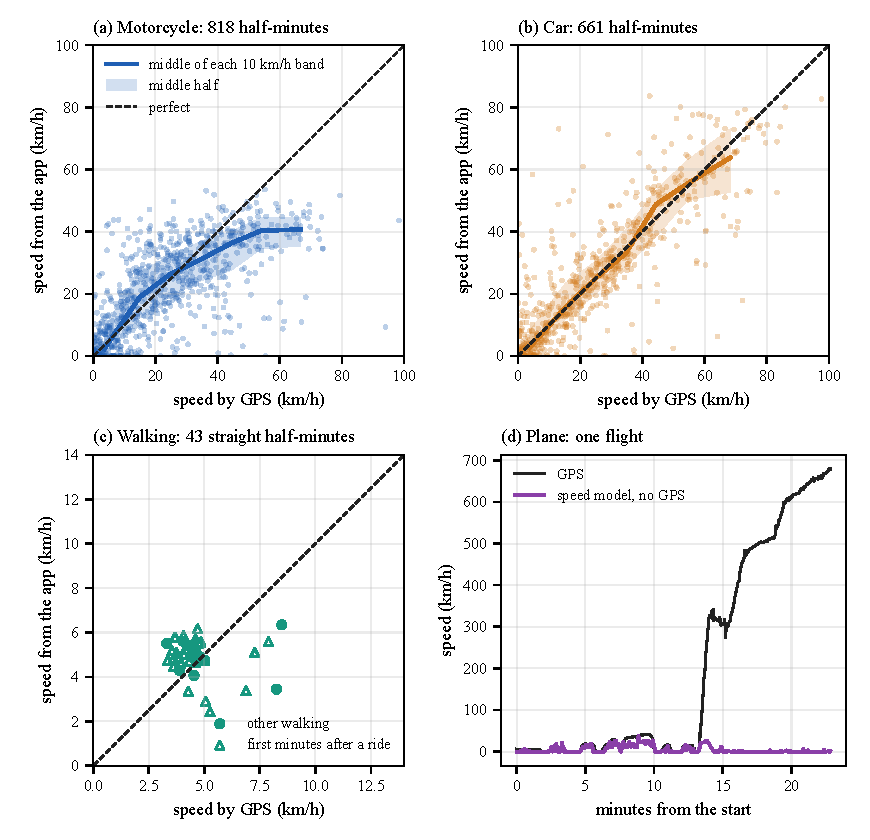
\includegraphics[width=0.66\textwidth]{figures/fig1_speed.pdf}
\caption{Speed from the system against speed from GPS, over $1457$ half-minutes of riding in
$70$ journeys. On the dashed line the two agree. The solid line is the middle of each $10$~km/h
band, and the shading holds the middle half of the readings.}
\label{fig:speed}
\end{figure}

Figure~\ref{fig:speed} shows the speed. Standing still and crawling are recognised correctly. In
between, the system squeezes the range: $10$--$30$~km/h reads about $2$--$4$~km/h high,
$30$--$40$~km/h is close, and above $60$~km/h it read about $49$ where GPS measured $67$. The average
error is about $9$~km/h. The squeeze comes from averaging twelve examples: when a fingerprint could
belong to several speeds, the average lands in the middle.

\subsection{Distance}

\begin{figure}[!htbp]
\centering
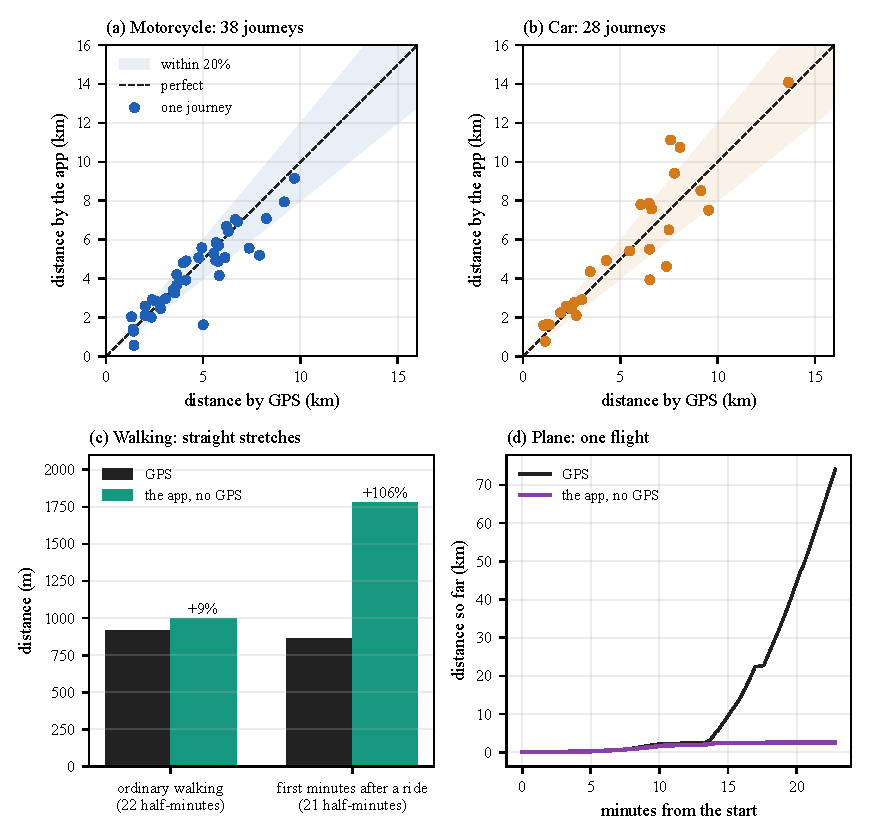
\includegraphics[width=0.92\textwidth]{figures/fig2_distance.pdf}
\caption{Distance for each of the $66$ journeys with at least $1$~km that GPS was good enough to
check. (a)~Each dot is one journey; on the dashed line the app and GPS agree. (b)~How far each
journey's distance is from GPS.}
\label{fig:distance}
\end{figure}

The over-reading at low speed and under-reading at high speed largely cancel over a journey.
Over the stretches GPS could check --- $318$~km in all --- the system added $314$~km, $1.5\%$
short. The middle journey was exactly right; $38\%$ of the journeys were within $10\%$ and $64\%$
within $20\%$ (Figure~\ref{fig:distance}). The worst were $68\%$ short and $54\%$ long.

\subsection{Direction}

\begin{figure}[!htbp]
\centering
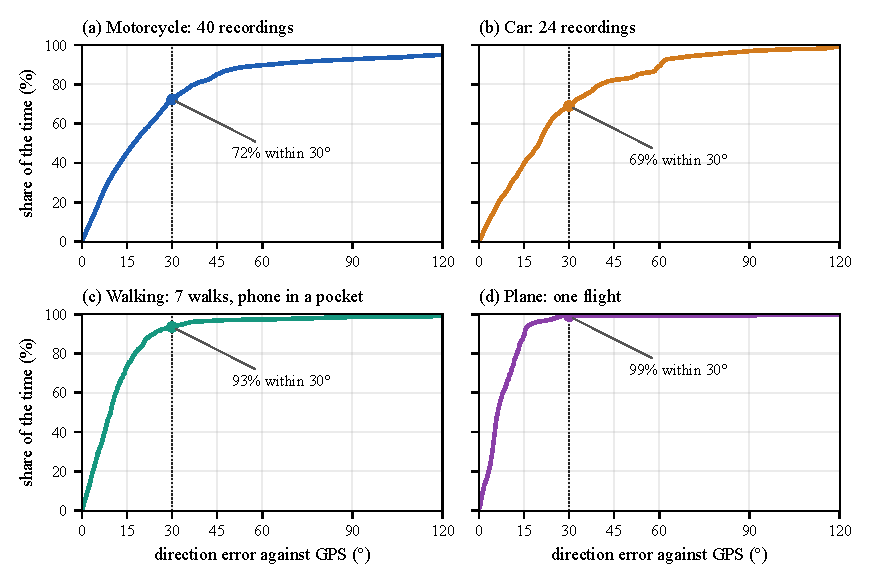
\includegraphics[width=0.92\textwidth]{figures/fig3_direction.pdf}
\caption{How often the direction is within a given angle of GPS. Left: $20{,}317$ seconds of
riding in $62$ recordings. Right: $721$ seconds of walking in seven walks, phone in a pocket.}
\label{fig:direction}
\end{figure}

While riding, the direction was within $30^\circ$ of GPS $73\%$ of the time and within
$45^\circ$ $85\%$ of the time; the middle error was $18^\circ$ (Figure~\ref{fig:direction}). While
walking with the phone in a pocket it was within $30^\circ$ $93\%$ of the time, with a middle
error of $10^\circ$.

\subsection{Whole routes}

\begin{figure}[!htbp]
\centering
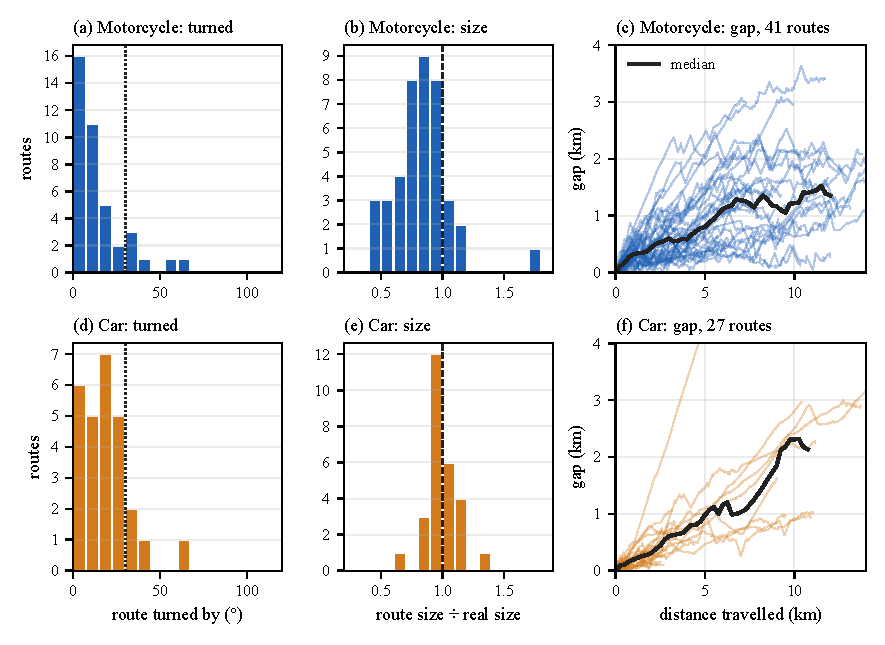
\includegraphics[width=\textwidth]{figures/fig4_routes.pdf}
\caption{$64$ routes drawn by the system, compared with GPS. (a)~How far each whole route is
turned from the GPS track; the dotted line is $30^\circ$. (b)~Its size relative to the GPS track.
(c)~How far the drawn position is from the GPS position as the journey goes on: one thin line per
route, and the median.}
\label{fig:routes}
\end{figure}

\begin{table}[!htbp]
\centering\small
\caption{Summary: the newest version against GPS.}
\label{tab:summary}
\begin{tabular}{lll}
\toprule
 & Measured over & Result\\
\midrule
Distance        & $70$ journeys, $318$~km & $1.5\%$ short in total; $64\%$ of journeys within $20\%$\\
Speed           & $1457$ half-minutes     & average error $9$~km/h\\
Direction, riding  & $62$ recordings      & within $30^\circ$ $73\%$ of the time\\
Direction, walking & $7$ walks            & within $30^\circ$ $93\%$ of the time\\
Direction, flight  & $1$ flight, $15$~min & within $30^\circ$ $99\%$ of the time\\
Route turned    & $64$ routes, $472$~km   & median $13^\circ$; $78\%$ within $30^\circ$\\
Route size      & $64$ routes             & median $0.95$; $69\%$ within $20\%$\\
Position gap    & $64$ routes             & median $17\%$ of the distance travelled\\
\bottomrule
\end{tabular}
\end{table}

Figure~\ref{fig:routes} and Table~\ref{tab:summary} put speed and direction together. The median
route is turned $13^\circ$ from the truth; $53\%$ are turned less than $15^\circ$ and $78\%$ less
than $30^\circ$. Drawn routes come out a little small --- a median $0.95$ of the real size --- even
though distance is about right, partly because small direction errors make the drawn path fold
slightly, so it ends nearer the start. The drawn position drifts away from GPS as the journey goes
on, by a median of about $17\%$ of the distance travelled: about $1.4$~km after $10$~km.

Six routes are turned more than $45^\circ$. Four of them are short journeys, under $3$~km,
with too few turns to learn the pocket angle well.

\subsection{A flight}

\begin{figure}[!htbp]
\centering
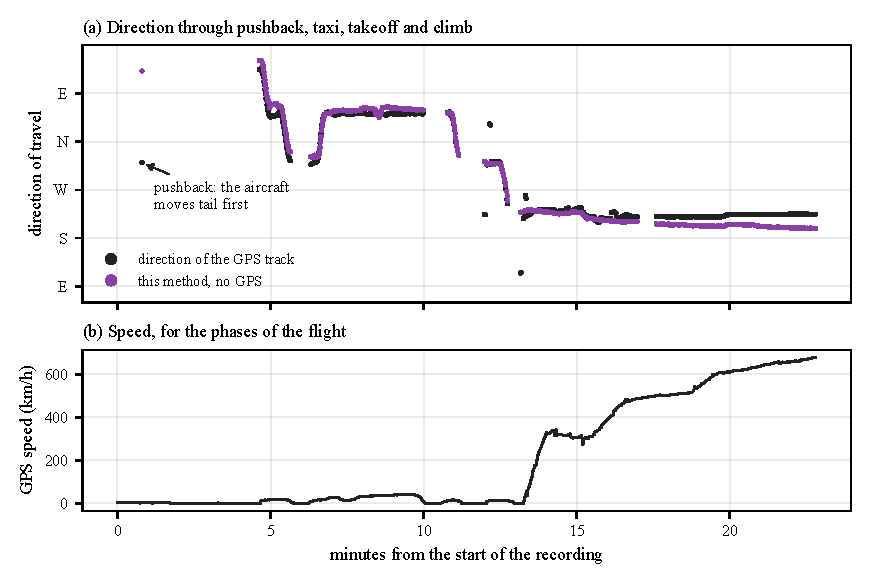
\includegraphics[width=0.92\textwidth]{figures/fig5_flight.pdf}
\caption{One flight, from the gate to the climb. (a)~The direction of travel from the GPS track
(black) and from this method, which uses no GPS (blue). (b)~The aircraft's speed from GPS, to show
where it was taxiing, taking off and climbing.}
\label{fig:flight}
\end{figure}

Figure~\ref{fig:flight} follows one flight with the same direction method as on the road. Speed
cannot be measured in an aircraft (Section~\ref{sec:wrong}), so only direction is compared. While
taxiing, the middle error was $8^\circ$; in the air it was $16^\circ$; over the whole recording the
direction was within $30^\circ$ of the GPS track $99\%$ of the time. The one large miss is the
pushback at the start, when the aircraft moves tail first: the method gives the way the nose points,
which is opposite to the way it moves. In the climb the gap grows slowly, to about $24^\circ$ by the
end of the recording. Part of that may be wind, which pushes an aircraft sideways so that its nose
and its track differ; GPS alone cannot tell the two apart.

\section{Where it goes wrong}\label{sec:wrong}

\begin{itemize}\itemsep2pt
\item \textbf{Fast riding reads slow, slow riding reads fast.} Above $60$~km/h the speed can be
half the true value (Figure~\ref{fig:speed}). Over a whole journey the two partly cancel, but a
journey that is mostly fast comes out short.
\item \textbf{The first minute of a ride.} Until the pocket angle is learned, the direction comes
from the compass alone, which in a pocket can be far off. The redrawing fixes the saved route
afterwards, but a very short ride may never learn the angle well.
\item \textbf{A phone that moves.} The pocket angle is assumed to stay the same for the whole
ride. If the phone shifts, the rest of the ride is turned by about as much as it moved. When the
phone is taken out of the pocket, the hand's movement hides the vehicle's vibration, so the last
speed is held; on one ride, $48$~km/h was held for ten seconds after the motorcycle had stopped,
about $130$~m that was never travelled.
\item \textbf{Car-park ramps.} A car crawling up a concrete ramp shakes like one driving at
$40$~km/h, so distance is not counted while climbing and turning together. The same test can
fire on an ordinary rising, curving road: once for nine seconds at $48$~km/h, about $115$~m lost.
\item \textbf{Aircraft.} Speed cannot be measured in an aircraft. The phone's own orientation
filter treats the long, steady push of a takeoff as a tilt~\cite{quatcf}, and the signal is gone.
The direction still works (Figure~\ref{fig:flight}).
\end{itemize}

\section{What did not work}

Many ideas were built and tested against GPS before the current version. The most instructive:

\begin{itemize}\itemsep2pt
\item \textbf{Neural networks.} A network that reads $20$--$40$ seconds of fingerprints at once
was more accurate on test data ($8.8$ against $10.6$~km/h) and ran in the app for a while, but
after it was retrained it under-read a pocketed ride by a third, and it was removed. Another
network, better than the current system on familiar data, was confidently wrong on a flight it
had never seen, recording $5\%$ of the distance, where the current system simply declines to
answer.
\item \textbf{Direction from speeding up and braking.} The push when accelerating in a straight
line points forward, so it should give direction. It was $44^\circ$ off; turns work far better.
\item \textbf{Other direction ideas}: the axis the motorcycle leans about ($25^\circ$ off), the
direction of the rider's thigh ($73^\circ$ off), and the swing of the thigh for telling forward
from backward when walking (wrong more often than right).
\item \textbf{How examples were forgotten.} When the store was full, it used to throw away
examples from whichever speed it held most of, to keep rare fast examples. That left it holding
$5\%$ of its examples below $5$~km/h when $24\%$ of real riding is that slow, so slow riding read
far too fast. Throwing away a random example instead fixed most of it.
\end{itemize}

\section{Lessons}

\begin{itemize}\itemsep2pt
\item \textbf{The phone's own definitions caused more error than the models.} Its built-in heading
becomes unreliable in a common pocket position, and its ``user acceleration'' points the opposite
way to the vehicle's acceleration. Each of these, once found, mattered more than any change to
the estimators.
\item \textbf{A test must not use what it is testing without.} Twice during development the
no-GPS test mode quietly used GPS for direction, which made its results look better than they
were.
\item \textbf{Check what a learning system remembers.} The store's way of forgetting examples was
sensible on its own and still shifted every answer, and it went unnoticed until its contents were
compared with the riding they came from.
\end{itemize}

\section*{Limits of this evaluation}

All recordings were made by one person, on one iPhone, mostly in one city, by motorcycle, car,
on foot and on one flight; other people, phones and vehicles may behave differently. Most results come from running the
newest method again over earlier recordings rather than from live use, though on the journeys the
app recorded with this version the rerun matched it closely. GPS in a pocket is itself only accurate
to tens of metres, so small errors cannot be measured reliably.

\begin{thebibliography}{9}
\small
\bibitem{carspeednet} A.~Cohen and I.~Klein. CarSpeedNet: Learning-based speed estimation from
accelerometer-only inertial sensing. arXiv:2401.07468, 2024.
\bibitem{memserrors} Smartphone MEMS accelerometer and gyroscope measurement errors: laboratory
testing and analysis of the effects on positioning performance. \emph{Sensors}, 23(17):7609, 2023.
\bibitem{pdrheading} Pedestrian dead reckoning with novel heading estimation under magnetic
interference and multiple smartphone postures. \emph{Measurement}, 183, 2021.
\bibitem{quatcf} Quaternion-based complementary filter for attitude determination of a
smartphone. \emph{IEEE Sensors Journal}, 16(15), 2016.
\end{thebibliography}

\end{document}
